\documentclass[conference]{IEEEtran}
\IEEEoverridecommandlockouts
\usepackage{cite}
\usepackage{amsmath,amssymb,amsfonts}
\usepackage{graphicx}
\usepackage{textcomp}
\usepackage{capt-of}
\usepackage{hyperref}
\hypersetup{
  colorlinks=true,
  allcolors=black,
  urlcolor=blue,
  citecolor=black,
  linkcolor=black
}
\usepackage{url}
\usepackage{xcolor}

% =====================================================================
% FLOAT PLACEMENT
%
% Table I, Table II and Fig. 2 are all inside ONE float environment, in
% that order. That is the only way to guarantee they stay together, in
% one column, in that sequence -- separate floats can always be split
% across columns or pages by the placement algorithm.
%
% Numbering is preserved: the two \caption calls step the table counter
% (Table I, Table II), and \captionof{figure} from capt-of steps the
% figure counter (Fig. 2). All four \label targets resolve normally.
%
% topnumber = 1 puts one float at each column top, so Fig. 1 takes the
% left column and the combined float takes the RIGHT column.
% =====================================================================
\setcounter{topnumber}{1}
\renewcommand{\topfraction}{0.95}
\setcounter{totalnumber}{2}
\renewcommand{\textfraction}{0.05}
\renewcommand{\floatpagefraction}{0.80}

\begin{document}

\title{Conformal-Gated Surrogate Screening for N-1 Under-Voltage Contingencies: Safety and Throughput Limits on a Marginally Secure Network}

\author{
\IEEEauthorblockN{Rajan Saha}
\IEEEauthorblockA{\textit{Conestoga High School}, Berwyn, PA, USA \\
\textit{Boston University RISE} \\
rajan.saha499@gmail.com}
\and
\IEEEauthorblockN{Eugene Pinsky}
\IEEEauthorblockA{\textit{Department\ of Computer Science} \\
\textit{Metropolitan College, Boston University} \\
epinsky@bu.edu}
}
\maketitle

\begin{abstract}
Electric power grids must stay secure after the loss of any single element. The so-called N-1 constraint requires an alternating-current (AC) power-flow solver for the loss of every component to compute the voltage of all the remaining equipment. With operators running every combination and repeatedly testing under different conditions, it becomes computationally expensive. Past work has replaced these solves with surrogates that check a group of cases at once, return a binary risk classification, or claim no missed unsafe scenarios with only a simple direct current (DC) model. In this study, we attach a one-sided split-conformal prediction interval to the predicted minimum post-contingency voltage for a ridge regression and a gradient-boosted model. Each model has three possible outputs: certify the situation as safe if the interval is above the 0.94 per-unit threshold, flag it if the prediction is below it, and escalate to the solver if the band straddles it. On the IEEE 118-bus AC network at 90\% coverage, the gradient-boosted model is 3.29 times faster than the solver but misses 4.72\% of violations. Reaching a sub-1\% missed rate results in a 64\% escalation and speedup dropping to roughly 1.6. In the IEEE 30-bus system, where 20.0\% of contingencies are near the limit rather than 56.9\% in the IEEE 118-bus system, a sub-1\% missed rate results in 8.96$\pm$0.91\% escalation at 11.27$\pm$1.02 times the solver's speed. These results allow operators to make an informed decision about whether surrogate screening would be worthwhile on a particular network.
\end{abstract}

\begin{IEEEkeywords}
contingency screening, conformal prediction, power-flow surrogate, selective prediction, power system security
\end{IEEEkeywords}

\section{Introduction}
Power grids must be able to stay operational even if they lose the functionality of a single element. The N-1 criterion, for all the elements that might fail, determines whether the calculated voltages of the remaining components stay within safe operating ranges after an element fails \cite{nerc}. Normally, the check itself comes from a physics calculation called an AC power flow solve, run for each potential contingency. For a complex network with hundreds of elements, the solver becomes time-consuming and computationally expensive.

One possible solution to improve performance is to replace the slow physics solver with a faster approximation. The main issue with this approach is not that it is inaccurate on average, but when it fails, it fails undetected, declaring an unsafe contingency safe, since it only provides a single-point estimate without an attached confidence or uncertainty interval \cite{bates2021}. As a result, the operator skips the slow solver and misses the unsafe scenario altogether. The error is asymmetric, as predicting too high certifies an unsafe condition as safe while predicting too low just wastes solver time. We keep track of the solver time for escalated cases and add it to the screening gate's total time to reflect the true end-to-end cost.

There have been several approaches when it comes to employing surrogate models for N-1 contingency tests. Manoharan \cite{manoharan2026} utilized a fast computer model that checks if any single piece of equipment in the N-1 test is in danger. To double-check reliability, the system also runs randomized full solves on some of the equipment it did skip to ensure the model is accurate. Alc\'antara and Chatzivasileiadis \cite{alcantara2026} use an AI foundation model and conformal prediction to create a binary yes/no switch for post-element outages to determine whether there's a present risk or not. Christianson et al. \cite{christianson2025} designed an input-convex network that completely removes false negatives, although that claim is only relevant to DC power flow models, not the AC power flow model our study uses. Our work stands out from these papers in three distinct ways. First, unlike the first two approaches, we add a band to each contingency. Second, we specifically check for only under-voltage issues. Finally, we explain why there must be a certain floor for escalation.

\section{Background}
A per-unit voltage normalizes power grid values into simple decimals (where 1.0 is nominal), where 0.94 per unit indicates a 6\% under-voltage. Utilities must keep voltage within a band around nominal, and this study flags any part of the grid that fails the test against an under-voltage floor of 0.94 per unit. The N-0 condition represents the current state of the grid without any equipment outages, in which all voltages are within safe limits. We refer to each pre-outage state of the grid as a base case. However, if a single piece of equipment fails, the rest of the network must absorb the extra load, which could cause the voltage to plunge below the safe 0.94 pu floor. N-1 screening simulates these failures and catches any violations of the under-voltage floor before they happen. In this study, we do not check for thermal line loading or over-voltage, so the only active constraint is the lower voltage limit.

An AC power flow solver is used to get the final voltages across a network after a single-element failure. Due to the math being complex and non-linear, it takes up to several milliseconds for one scenario, and the time multiplies across the whole grid. By contrast, a prediction from a machine learning model can take a fraction of a millisecond for predicting the single minimum voltage out of the whole grid. Classical fast screens rank power system contingencies without running a full solver \cite{ejebe1979}. While this indicates which equipment is subject to the most danger when there's an equipment failure, it fails to provide a numerical minimum voltage.

We study the IEEE 118-bus system \cite{case118}, a standard electrical power test case with 118 buses (the junctions where voltage is measured), 173 lines, and 13 transformers. Since our N-1 test set includes only lines and transformers, there are 186 total pieces of equipment that are subject to failure. We use pandapower \cite{pandapower}, a Python library used to model power systems, for solving post-outage voltages while ensuring specific generator reactive power limits are enforced.

\section{Method}
\subsection{Dataset}
We determined the load and generation levels by multiplying the load and generator base values by multipliers ranging uniformly from 1.0 to 1.12. The base cases were kept if the minimum pre-outage voltage exceeded 0.94 per unit, with only 53.82\% of the cases passing this. Each accepted base case was put through a simulation of 186 contingencies representing single-element failures, followed by an alternating-current power flow calculation to determine the minimum bus voltage after each contingency. The total sample contained 1{,}500 base cases and 280{,}500 rows, including the base cases. 278{,}955 of these solved successfully, with the remainder failing to converge and, as a result, removed. Post-contingency voltages ranged from 0.7179 to 0.9603 per unit, and 17.48\% of the observations violated the voltage limit. We also tested the IEEE 30-bus system, and since there are 41 rather than 186 branches, the 1{,}500 bases produce 61{,}500 contingency scenarios, all of which were solved successfully.

\subsection{Surrogates}
The surrogate predicts the minimum voltage following an outage based on the per-bus loads, how generators are set up, baseline voltages, and the failed equipment. The two algorithms used in this study are a ridge linear regression model using standardized inputs and a histogram-based gradient-boosted tree ensemble \cite{sklearn}. The data is split into 60\%, 20\%, and 20\% sets using different base scenarios for training, calibration, and test sets, respectively. To pick the settings for each model, we split the training set again into three smaller parts: one to fit the model, one to calculate the band width $\hat{q}$, and one to test the gate on. We never look at the real calibration or test sets while choosing settings. Instead, we keep whichever settings skip the most solves while still missing 1\% or fewer of the violations, and we repeat the whole process with five different random splits. We test our models against two baselines: persistence, which predicts the pre-outage minimum voltage, and the training mean.

\subsection{One-sided conformal band}
The split-conformal prediction approach converts the residuals from the calibration dataset into a coverage guarantee (the number of cases the band is guaranteed to contain)\cite{lei2018,vovk2005}. Since the primary source of the danger is the voltage being less than the predicted one, we compute only the lower band. It is specified via $\hat{q}$ as the quantile for the coverage of the model overshoot (the difference between the prediction and the true value) based on the finite-sample rank approach proposed by Lei et al.\ \cite{lei2018} and form the one-sided band
\begin{equation}
\text{lower} = \hat{p} - \hat{q},
\end{equation}
where $\hat{p}$ is the prediction. As long as the test cases and calibration cases come from the same type of condition (a single-element outage), the true voltage remains at or above the lower bound with the desired probability. If this condition does not hold (i.e., using calibration data of a single-element outage with test data of a two-element outage), there is no guarantee for what the band truly encompasses, which raises the issue of distribution shift described in Section~V. A single quantile coverage is the easiest way to choose the band, and locally adaptive alternatives exist \cite{romano2019}. At a 90\% coverage level, the calibrated band widths are 0.0052 per unit for the linear model and 0.0023 per unit for the gradient-boosted model.

\subsection{Three-way gate}
For each contingency, the gate performs the following tests for the band and the point prediction compared with the limit $L=0.94$:
\begin{itemize}
\item \textbf{Certify} (skip the solver): $\hat{p}-\hat{q}\ge L$, meaning that the lower edge of the band exceeds the limit.
\item \textbf{Flag} (skip the solver): $\hat{p}< L$, meaning that the point prediction itself is below the limit.
\item \textbf{Escalate} (invoke the solver) otherwise, that is, when the band straddles the limit.
\end{itemize}
The flagging test employs the point prediction rather than the lower edge of the band since the one-sided band has no upper edge (Fig.~\ref{fig:gate}). The exact solver is invoked on escalations only; the net speedup accounts for that cost:
\begin{equation}
\text{net speedup} = \frac{n\, t_{\text{solve}}}{n\, t_{\text{surr}} + n_{\text{esc}}\, t_{\text{solve}}}
\end{equation}
Here $n$ is the total number of contingencies, $t_{\text{solve}}$ is the solver time per case (set at 9.14 ms, which is the minimum over 400 timed solves), $t_{\text{surr}}$ is the surrogate time, and $n_{\text{esc}}$ is the escalation count. The net speedup is close to the inverse of the escalation rate since the surrogate is much cheaper than the solve.

% =====================================================================
% FIGURE 1 (fig:gate) -- gate schematic. Cited in III-D.
% Takes the LEFT-column top; with topnumber=1 this is what forces the
% combined table/figure float into the RIGHT column.
% =====================================================================
\begin{figure}[!t]
\centerline{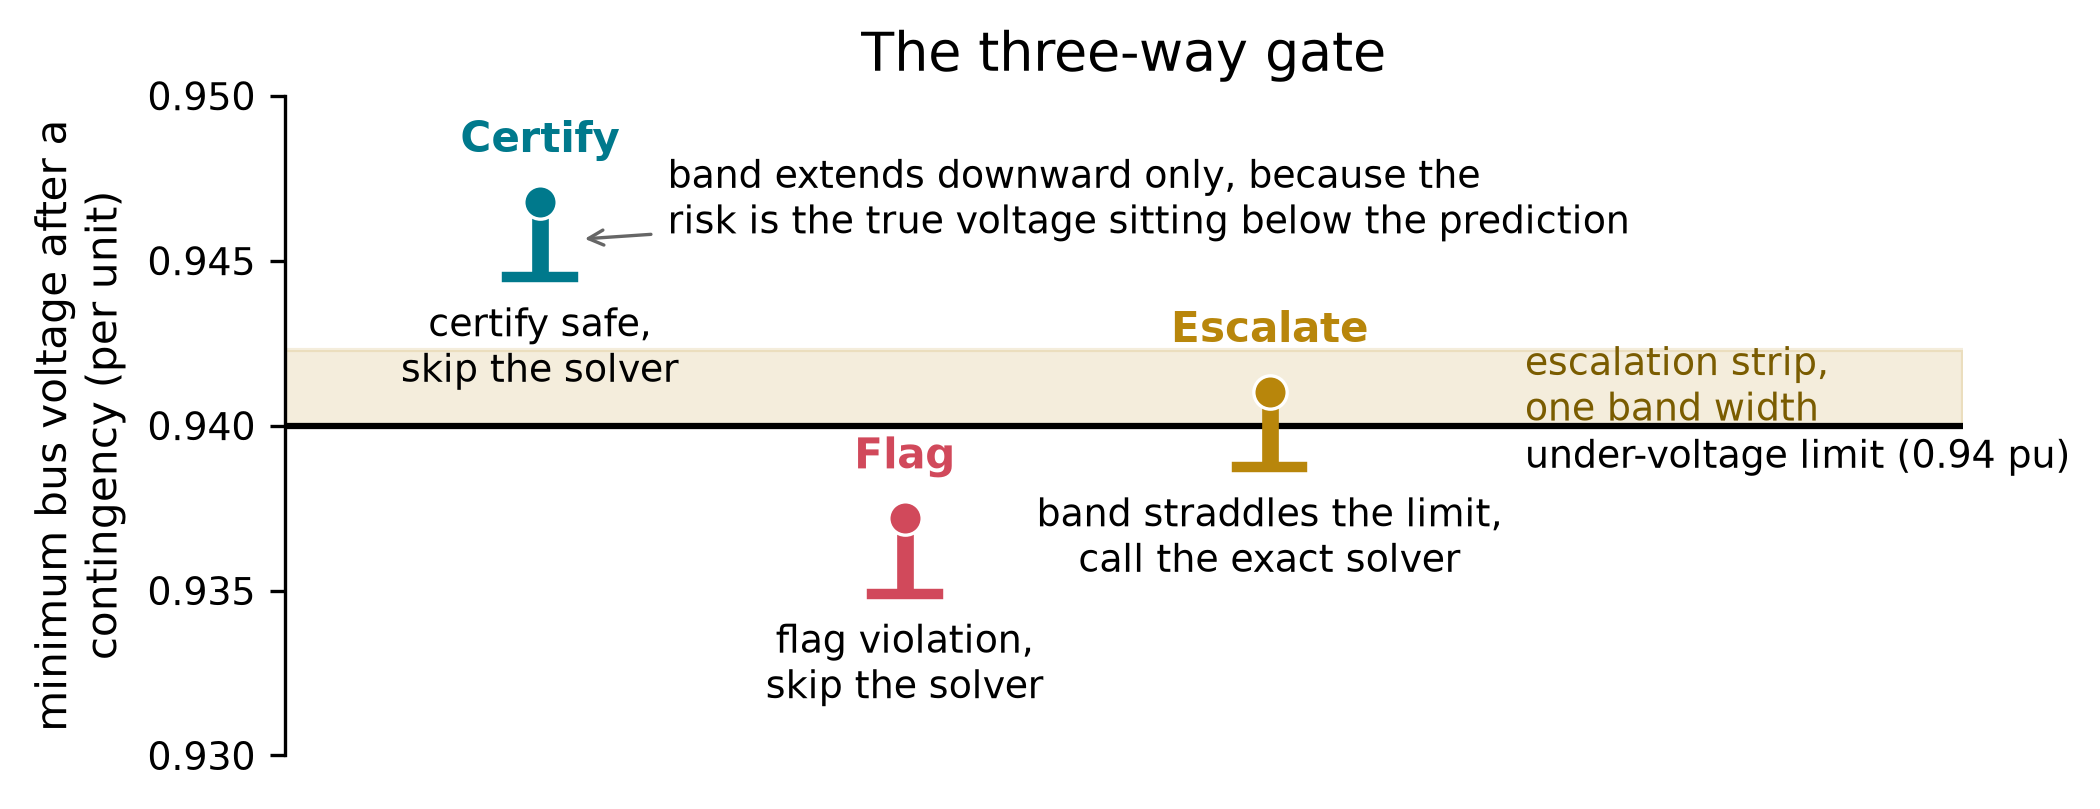
\includegraphics[width=\columnwidth]{data/gate_schematic_v2.png}}
\caption{The surrogate predicts post-outage voltage and attaches a band extending only downward. A case is certified if the whole band clears 0.94 pu, flagged if the prediction falls below it, and escalated if the band straddles it.}
\label{fig:gate}
\end{figure}

% =====================================================================
% COMBINED FLOAT: TABLE I, then TABLE II, then FIGURE 2.
%
% TABLE I (tab:models): v2 PROMOTED bodies. persistence and train-mean
% rows are copied verbatim from the committed models and are
% byte-identical. Column spec lccccc, 6 fields. tabcolsep dropped from
% 3pt to 1pt: at 3pt this table overran the column and the Speedup
% column bled into the neighbouring text.
%
% TABLE II (tab:ops): v2 PROMOTED (M2 gate-aware tuned) bodies, from
% notes/paper_tables_v2.tex, generated by scripts/emit_v2_tables.py from
% data/tradeoff_curve_v2.json. Column spec llcccc, 6 fields.
%
% FIGURE 2 (fig:tradeoff): coverage sweep, data/tradeoff_hero_col_v2.png.
% Uses \captionof{figure} so it numbers on the FIGURE counter even though
% the enclosing environment is a table float.
%
% Estimated combined height is roughly two thirds of a column, so this
% should place at a column top rather than spilling to a float page.
% =====================================================================
\begin{table}[!t]
\caption{Four-model comparison at 90\% target coverage. Means $\pm$ standard deviation over five random splits. Escalation and missed-violation rate (share of true violations) in percent; histgb is the gradient-boosted model. $^{\dagger}$The train-mean model never calls the solver, so this does not represent a proper screening speedup.}
\label{tab:models}
\centering
\footnotesize
\setlength{\tabcolsep}{1pt}
\begin{tabular}{lccccc}
\hline
Model & MAE ($10^{-3}$ pu) & $R^2$ & Esc. & Missed & Speedup \\
\hline
persistence & 4.2$\pm$0.1 & $-0.06\pm0.00$ & 99.5$\pm$0.2 & 0.31$\pm$0.08 & 1.00$\pm$0.00 \\
train mean  & 6.7$\pm$0.2 & $-0.00\pm0.00$ & 0.0$\pm$0.0 & 0.00$\pm$0.00 & N/A$^{\dagger}$ \\
ridge       & 3.8$\pm$0.1 & 0.77$\pm$0.01 & 49.1$\pm$2.7 & 2.96$\pm$0.44 & 2.04$\pm$0.11 \\
histgb      & 1.6$\pm$0.1 & 0.92$\pm$0.00 & 30.6$\pm$2.5 & 4.72$\pm$0.98 & 3.29$\pm$0.30 \\
\hline
\end{tabular}

\vspace{3ex}

\caption{Safety and throughput at each coverage target on IEEE 118-bus system. Means $\pm$ standard deviation over five random splits. Escalation, empirical coverage, and missed-violation rate (share of true violations) in percent; histgb is the gradient-boosted model.}
\label{tab:ops}
\centering
\footnotesize
\setlength{\tabcolsep}{3pt}
\begin{tabular}{llcccc}
\hline
Model & Target & Esc. & Cov. & Missed & Speedup \\
\hline
ridge  & 0.90 & 49.1$\pm$2.7 & 89.3$\pm$1.3 & 2.96$\pm$0.44 & 2.04$\pm$0.11 \\
ridge  & 0.94 & 64.3$\pm$2.8 & 94.0$\pm$0.7 & 0.79$\pm$0.21 & 1.56$\pm$0.07 \\
ridge  & 0.95 & 67.9$\pm$2.8 & 95.0$\pm$0.6 & 0.45$\pm$0.12 & 1.48$\pm$0.06 \\
ridge  & 0.96 & 71.4$\pm$1.4 & 95.9$\pm$0.4 & 0.14$\pm$0.07 & 1.40$\pm$0.03 \\
ridge  & 0.97 & 73.9$\pm$1.0 & 96.9$\pm$0.2 & 0.03$\pm$0.03 & 1.35$\pm$0.02 \\
ridge  & 0.98 & 74.8$\pm$0.8 & 98.0$\pm$0.2 & 0.00$\pm$0.00 & 1.34$\pm$0.01 \\
histgb & 0.90 & 30.6$\pm$2.5 & 89.8$\pm$1.0 & 4.72$\pm$0.98 & 3.29$\pm$0.30 \\
histgb & 0.94 & 46.7$\pm$2.8 & 93.7$\pm$0.4 & 2.48$\pm$0.38 & 2.15$\pm$0.13 \\
histgb & 0.95 & 51.2$\pm$3.4 & 94.7$\pm$0.4 & 1.94$\pm$0.21 & 1.96$\pm$0.13 \\
histgb & 0.96 & 57.0$\pm$4.3 & 95.7$\pm$0.4 & 1.36$\pm$0.20 & 1.76$\pm$0.12 \\
histgb & 0.97 & 63.7$\pm$5.1 & 97.0$\pm$0.2 & 0.83$\pm$0.24 & 1.58$\pm$0.12 \\
histgb & 0.98 & 72.0$\pm$3.7 & 98.0$\pm$0.2 & 0.30$\pm$0.13 & 1.39$\pm$0.07 \\
\hline
\end{tabular}

\vspace{3ex}

\centerline{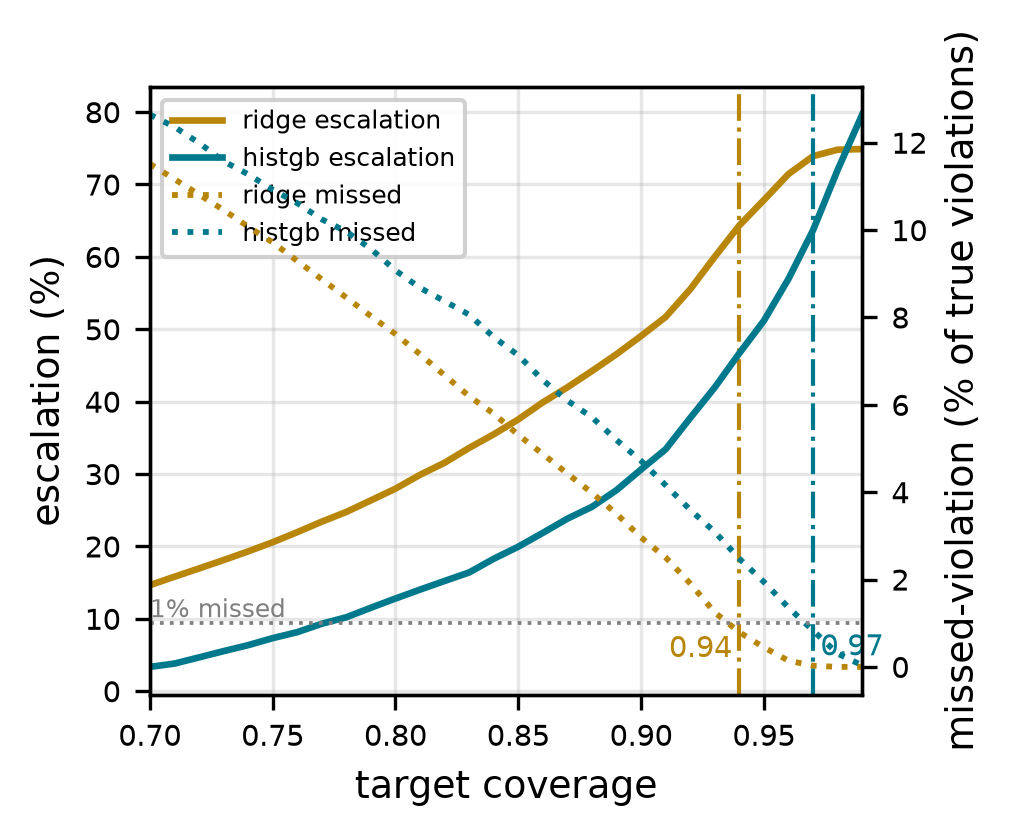
\includegraphics[width=\columnwidth]{data/tradeoff_hero_col_v2.png}}
\captionof{figure}{Escalation (solid, left axis) and missed violations (dotted, right axis) are plotted against the safety target and averaged over five splits. The missed rate first falls below 1\% at 0.94 coverage for ridge and 0.97 for the gradient-boosted model, with high escalation at both.}
\label{fig:tradeoff}
\end{table}

\section{Results}
Both surrogates accurately predict the minimum post-contingency voltage for the gate to work. The linear model reaches an $R^2$ of 0.77 and the gradient-boosted model 0.92, with mean absolute errors of 0.0038 and 0.0016 per unit, respectively (Table~\ref{tab:models}). At 90\% coverage, the ridge model escalates 49.1\% of cases, has 89.3\% coverage, misses 2.96\% of violations, and is 2.04 times faster than the solver. The gradient-boosted model escalates 30.6\%, has 89.8\% coverage, and is 3.29 times faster than the solver, yet it misses 4.72\% of violations. Both models ensure that the band is calibrated, as the coverage is close to 90\%. The problem of safety does not lie in how much error there is, but in where that error falls.

\subsection{Safety comes at high escalation}
In Table~\ref{tab:ops}, we adjusted the target from 0.90 to 0.98 and recorded the missed and escalation rates. Increasing the target decreases the missed rate but also increases the escalation rate, as the larger band size needed to cover potential model overshooting makes it more likely to straddle the threshold. For the gradient-boosted model, increasing the target from 0.90 to 0.94 decreases the missed rate from 4.72\% to 2.48\%, increases the escalation from 30.6\% to 46.7\%, and decreases the speed-up from 3.29 to 2.15 times. The ridge model behaves similarly, with a missed rate below 1\% occurring first at 0.94 for the ridge model (0.79\% missed, 64.3\% escalation, 1.56 times faster) and 0.97 for the gradient-boosted model (0.83\% missed, 63.7\% escalation, 1.58 times faster), as Fig.~\ref{fig:tradeoff} shows.

% =====================================================================
% FIGURE 3 (fig:missdepth) -- miss-depth histogram, from
% data/miss_depth_v2.png (log-y; generated by scripts/miss_depth_fig.py
% from data/missed_depth.json). Cited in IV-B.
% Upload the PNG to the Overleaf data/ folder or this will not resolve.
% =====================================================================
\begin{figure}[!t]
\centerline{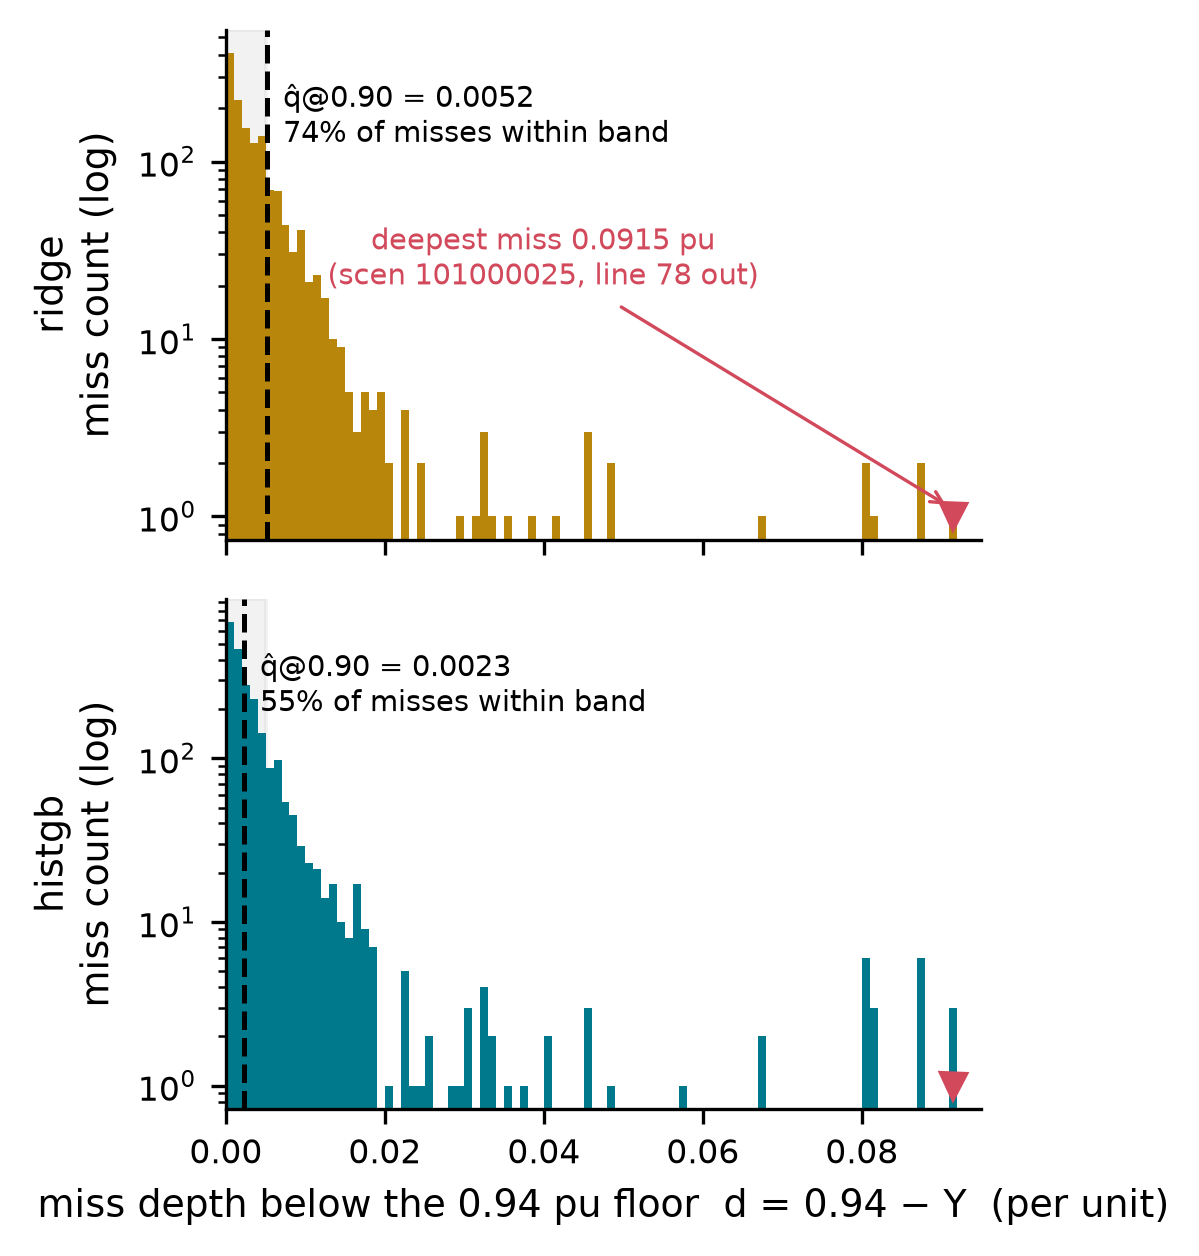
\includegraphics[width=\columnwidth]{data/miss_depth_v2.png}}
\caption{The histogram measures how far missed violations fall below 0.94 pu at 90\% coverage on a logarithmic count scale. Dashed lines mark each model's band width. Most misses stay within one band, but a thin tail reaches 0.0915 pu, where one certified bus had fallen to 0.8485.}
\label{fig:missdepth}
\end{figure}

\subsection{The faster model is not the safer one}
The choice of which model to use changes along the coverage axis, and Table~\ref{tab:models} shows that accuracy cannot settle this decision by itself. The gradient-boosted model is far more accurate than the linear one, and at 0.90 coverage it is also faster, with it being 3.29 times faster versus 2.04 times. However, when we consider safety, we notice that at a coverage of 0.96, the linear model misses 0.14\% of the violations while the gradient-boosted model misses 1.36\%. The linear model also demonstrates the lower missed rate across all targets in the sweep. The model's errors differ in terms of frequency and depth, as at 0.90 coverage, 74\% of misses fall within one band width of the limit for the linear model and 55\% for the gradient-boosted model (Fig.~\ref{fig:missdepth}). Only a few misses were serious, with the worst being 0.0915 per unit under the limit, which was a bus that fell to 0.8485.

\subsection{The boundary layer sets a floor on escalation}
The majority of contingencies are within 0.005 per unit of the boundary, which results in a large amount of escalations. Fig.~\ref{fig:boundary} provides a histogram of voltages following contingencies. Out of all the converged cases, 56.86\% are in a narrow range of [0.94, 0.945), slightly higher than the threshold, and 17.48\% lie below the threshold as violations. Notably, no 0.001-per-unit width bin makes up more than around 14\% of the entire dataset. Certain buses account for extreme events, with bus 76 being the weakest one, holding the minimum voltage in 27.1\% of contingencies, whereas bus 53 is second with 16.81\%, followed by bus 107 with 9.31\%.

% =====================================================================
% FIGURE 4 (fig:boundary) -- boundary-mass histogram, from
% data/boundary_mass_hist.png. Cited in IV-C.
% =====================================================================
\begin{figure}[!t]
\centerline{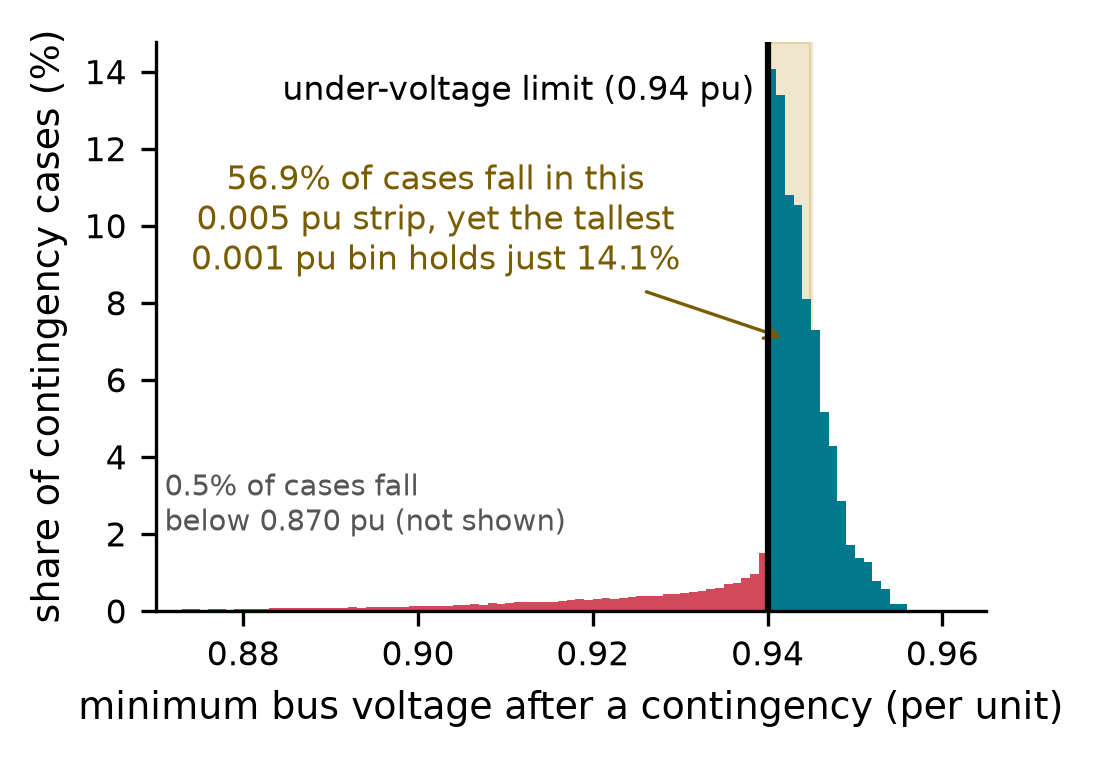
\includegraphics[width=\columnwidth]{data/boundary_mass_hist.png}}
\caption{Lowest voltage across all failure cases; anything left under the line is a violation. Over half are within 0.005 pu above the limit, while the tail below the limit drops much lower.}
\label{fig:boundary}
\end{figure}

A case is escalated when its prediction lands within one band width above this limit. The gradient-boosted model's band is only 0.0023 pu wide, but so much of the distribution sits just above 0.94 that this narrow window still captures 30.6\% of all contingencies. As the band becomes larger, escalation moves closer to every case predicted at or above the limit, the remaining 82.52\% of cases, or the saturation point. Linear prediction overpredicts cases below the limit compared to gradient-boosted prediction, and thus has a lower escalation ceiling of 74.9\% versus 82.8\%. The gradient-boosted model flags violations about as often as they occur, so its ceiling essentially lands on the saturation point. A model that rarely predicts below the limit has a higher ceiling and misses more violations.

Persistence is a baseline model that assumes the voltage before the single-element outage equals the voltage afterwards. All the pre-outage scenarios are above 0.94 pu, so its predictions never go below the limit, and since it cannot predict under the limit, it can never mark a case as a violation. In Table~\ref{tab:models}, the model escalates 99.5\% of cases and is barely faster than the solver in terms of time taken. To decrease the escalation rate, the model must validate cases as safe, but also risk misclassifying some as well. An operator that requires a sub-1\% missed rate would run the models at a 0.94 or a 0.97 target coverage and accept about a 1.6 times speedup instead of the 2 to 3 times available at 0.90.

\section{Discussion and limitations}
The core ideas of calibrated uncertainty and deciding whether or not to hand over the task to a more complex model \cite{desalvo2015}, or giving the model multiple options \cite{angelopoulos2024,cortes2016,chow1970} are established methods. In our study, two things differ from that literature. First, we fall back to an exact solver instead of a more complex model, so the escalated case can be resolved, and second, we also explain why the speedup is capped, which is because most of the data is very close to the limit.

Our approach differs from Manoharan's audited population control \cite{manoharan2026}, which is itself a form of distribution-free risk control \cite{bates2021}. His method uses a bound for the proportion of skipped cases that are unsafe, while our gate uses a margin of error that is subtracted from each prediction. This introduces the lower bound, since split conformal prediction allows us to be correct on average but not necessarily within the band. If one demands perfect correctness with a limited amount of calibration data, then the prediction intervals become extremely wide, to the point where it becomes useless \cite{barber2021}. Every base case generates 186 related contingencies, and therefore, the coverage rates are measured averages rather than guarantees on individual contingencies.

The main experimental results use one network with realistic topology but synthetic loads and generation levels. The floor exists on any network, but its height depends on the data distribution. For example, on the IEEE 30-bus network simulated using the same configuration, 20.0\% of contingencies approach the threshold, whereas another 28.8\% fall below it, so the same missed rate gives 8.96$\pm$0.91\% escalations and an 11.27$\pm$1.02 times speedup. The ANSI C84.1 Range B specification \cite{ansi2020} allows service voltages down to 0.917 pu, though it governs service rather than transmission voltage. We use 0.94 pu as a conservative choice, and it also fits how the pre-outage data is distributed. Only 86 of the 1,500 base cases are above 0.95 pu, while all sit above 0.94 pu. Increasing the threshold to 0.95 pu leads to an escalation of roughly 1.5\%. In other words, the method flags almost all instances as unsafe, offering nothing to operators.

Our claims of safety are only true for N-1 contingency cases, since we did not test N-2 cases. In addition, mathematical proof is unable to determine the safety of N-2 outages since conformal prediction requires the data to be exchangeable with the calibration set \cite{tibshirani2019}. Also, we only checked if the final voltage was too low, not for thermal overheating, over-voltage, or whether or not the grid crashed in the first place, which is called dynamic stability. The band only counts instances of where the model is wrong and not how badly it fails. In addition, the worst case, at 0.0915 per unit, is an example of a sudden collapse where a generator at that case's weakest bus hits its reactive limit and can no longer regulate voltage. A model trained only on pre-outage features cannot predict such a situation. Finally, all of the testing data was generated from small variations around one pre-contingency grid setup, so we are unsure of the frequency or timing at which operators should recalibrate the models as seasons and demand change throughout the year.

\section{Conclusion and future work}
Our models can predict N-1 under-voltage contingencies on the IEEE 118-bus system. On this network, safety and speed are inversely related, though the 30-bus result shows that this depends on data distribution relative to the limit. At 90\% coverage, the models are fast but miss too many contingencies, and to bring the missed rate below 1\% requires escalating around two-thirds of cases, and the speedup on this network decreases enough to be comparable to the speed of the solver itself. The main reason is that most of the cases fall very close to the limit. As a result, the bands often straddle this limit and then must escalate to the solver as the result is uncertain. Our contribution is explaining why that floor exists, and a note of caution to anyone expecting large speedups from a surrogate that must be safe on every case. Future work includes testing multiple-element outages and a third network to see whether the speedup achieved correlates with how many contingencies lie near the limit.

\section*{Acknowledgments}
This paper has been written as part of the Boston University RISE data science practicum. The authors would like to thank the program and the teaching fellows and staff. An AI assistant, Claude from Anthropic, was used to validate the code and grammar. All reported numbers were generated using the authors' committed and tested code that is available at the following link: \url{https://github.com/rajsaha-blip/contingency-screener-research}. 

% =====================================================================
% References. arXiv entries verified in notes/prior-art.md; the classic and
% software entries were fetch-verified on 2026-07-21 (dblp, IEEE Xplore,
% Oxford Academic, NeurIPS proceedings, JMLR, UW test-case archive); the two
% ALT conference entries (cortes2016, desalvo2015) on 2026-07-23 (Crossref + dblp;
% Springer chapter pages behind an auth wall); bates2021 from the publisher
% PDF; tibshirani2019 on 2026-07-26 (NeurIPS proceedings page + ACM DL);
% angelopoulos2024, christianson2025 and ansi2020 on 2026-07-29 (medRxiv full
% text, proceedings.mlr.press/v283/christianson25a.html, and the NEMA official
% excerpt respectively). No field is filled from memory.
% =====================================================================
\begin{thebibliography}{19}
\bibitem{nerc} \textit{Transmission System Planning Performance Requirements}, NERC Reliability Standard TPL-001-5.1, North American Electric Reliability Corporation, Atlanta, GA, USA, eff. Jul. 1, 2023.
\bibitem{bates2021} S. Bates, A. Angelopoulos, L. Lei, J. Malik, and M. Jordan, ``Distribution-free, risk-controlling prediction sets,'' \textit{J. ACM}, vol. 68, no. 6, art. 43, 2021.
\bibitem{manoharan2026} J. Manoharan, ``Audited selective verification for risk-controlled N-1 thermal contingency screening under deployment shift,'' arXiv:2607.13221, 2026.
\bibitem{alcantara2026} A. Alc\'antara and S. Chatzivasileiadis, ``Trustworthiness layer for foundation models in power systems: Application to N-k contingency screening,'' arXiv:2602.07995v2, 2026.
\bibitem{christianson2025} N. Christianson, W. Cui, S. Low, W. Yang, and B. Zhang, ``Fast and reliable N-k contingency screening with input-convex neural networks,'' in \textit{Proc. 7th Annu. Learn. Dynamics Control Conf. (L4DC)}, ser. PMLR, vol. 283, 2025, pp. 527--539.
\bibitem{ejebe1979} G. C. Ejebe and B. F. Wollenberg, ``Automatic contingency selection,'' \textit{IEEE Trans. Power App. Syst.}, vol. PAS-98, no. 1, pp. 97--109, 1979.
\bibitem{case118} R. Christie, ``Power systems test case archive: IEEE 118-bus system,'' Univ. of Washington, 1993. [Online]. Available: https://labs.ece.uw.edu/pstca/
\bibitem{pandapower} L. Thurner, A. Scheidler, F. Sch\"afer, \textit{et al.}, ``pandapower---an open-source Python tool for convenient modeling, analysis, and optimization of electric power systems,'' \textit{IEEE Trans. Power Syst.}, vol. 33, no. 6, pp. 6510--6521, Nov. 2018.
\bibitem{sklearn} F. Pedregosa \textit{et al.}, ``Scikit-learn: Machine learning in Python,'' \textit{J. Mach. Learn. Res.}, vol. 12, pp. 2825--2830, 2011.
\bibitem{lei2018} J. Lei, M. G'Sell, A. Rinaldo, R. J. Tibshirani, and L. Wasserman, ``Distribution-free predictive inference for regression,'' \textit{J. Amer. Statist. Assoc.}, vol. 113, no. 523, pp. 1094--1111, 2018.
\bibitem{vovk2005} V. Vovk, A. Gammerman, and G. Shafer, \textit{Algorithmic Learning in a Random World}. New York, NY, USA: Springer, 2005.
\bibitem{romano2019} Y. Romano, E. Patterson, and E. J. Cand\`es, ``Conformalized quantile regression,'' in \textit{Adv. Neural Inf. Process. Syst. (NeurIPS)}, vol. 32, 2019, pp. 3538--3548.
\bibitem{barber2021} R. F. Barber, E. J. Cand\`es, A. Ramdas, and R. J. Tibshirani, ``The limits of distribution-free conditional predictive inference,'' \textit{Inf. Inference: J. IMA}, vol. 10, no. 2, pp. 455--482, 2021.
\bibitem{desalvo2015} G. DeSalvo, M. Mohri, and U. Syed, ``Learning with deep cascades,'' in \textit{Algorithmic Learning Theory (ALT)}, ser. Lecture Notes in Comput. Sci., vol. 9355. Springer, 2015, pp. 254--269.
\bibitem{angelopoulos2024} A. N. Angelopoulos \textit{et al.}, ``Conformal triage for medical imaging AI deployment,'' medRxiv, 2024, doi: 10.1101/2024.02.09.24302543.
\bibitem{cortes2016} C. Cortes, G. DeSalvo, and M. Mohri, ``Learning with rejection,'' in \textit{Algorithmic Learning Theory (ALT)}, ser. Lecture Notes in Comput. Sci., vol. 9925. Springer, 2016, pp. 67--82.
\bibitem{chow1970} C. K. Chow, ``On optimum recognition error and reject tradeoff,'' \textit{IEEE Trans. Inf. Theory}, vol. 16, no. 1, pp. 41--46, 1970.
\bibitem{tibshirani2019} R. J. Tibshirani, R. Foygel Barber, E. J. Cand\`es, and A. Ramdas, ``Conformal prediction under covariate shift,'' in \textit{Adv. Neural Inf. Process. Syst. (NeurIPS)}, vol. 32, 2019, pp. 2526--2536.
\bibitem{ansi2020} \textit{American National Standard for Electric Power Systems and Equipment---Voltage Ratings (60~Hz)}, ANSI Standard C84.1-2020, National Electrical Manufacturers Association, Rosslyn, VA, USA, 2020.
\end{thebibliography}

\end{document}